\section{The model}
  Restricted Boltzmann Machines are a model used mainly for unsupervised learning. We collect
  data from an unknown distribution and then use it to set the parameters of the RBM to match
  the starting distribution as closely as possible.
  
  \subsection{General RBM}
  Consider a fully-connected bipartite undirected graph as shown in Figure~\ref{fig:generalRBM}.
  It consists of \emph{visible} layer with $m$ nodes labeled by \(V_1, \dots, V_m\) and a
  \emph{hidden} layer whose \(n\) nodes are labeled by \(H_1, \dots, H_n\). We call \(\mathcal{V}\)
  the set of visible nodes, and \(\mathcal{H}\) the set of hidden nodes.
  \begin{figure}
    \centering
    \resizebox{\textwidth}{!}{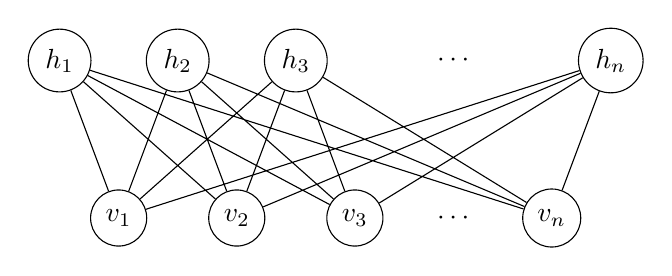
\begin{tikzpicture}%[node distance={15mm}, thick, main/.style = {draw, circle}] 
  \node[draw, circle] (h1) at (1.5,1)   {$h_1$}; 
  \node[draw, circle] (h2) at (3,1)   {$h_2$};
  \node[draw, circle] (h3) at (4.5,1)   {$h_3$};
  \node            (hdots) at (6.5,1) {$\cdots$};
  \node[draw, circle] (hn) at (8.5,1)   {$h_n$};
  
  \node[draw, circle] (v1) at (2.25,-1)   {$v_1$}; 
  \node[draw, circle] (v2) at (3.75,-1)   {$v_2$};
  \node[draw, circle] (v3) at (5.25,-1)   {$v_3$};
  \node            (vdots) at (6.5,-1) {$\cdots$};
  \node[draw, circle] (vm) at (7.75,-1)   {$v_n$};
  
  \draw (v1)--(h1)
        (v1)--(h2)
        (v1)--(h3)
        (v1)--(hn)
        (v2)--(h1)
        (v2)--(h2)
        (v2)--(h3)
        (v2)--(hn)
        (v3)--(h1)
        (v3)--(h2)
        (v3)--(h3)
        (v3)--(hn)
        (vm)--(h1)
        (vm)--(h2)
        (vm)--(h3)
        (vm)--(hn);
\end{tikzpicture} }
    \caption{An RBM graph with \(n\) hidden and \(m\) visible nodes.}
    \label{fig:generalRBM}
  \end{figure}
  Let us consider a random variable \(X_U\) associated with a node \(U\) (either visible or hidden)
  that takes values in \(\Lambda_U\). We say that our graph satisfies the \emph{Markov
  property} if 
  \begin{align*}
    \CondProb{X_v}{\{X_{v'}\}_{v'\in (\mathcal{V} \setminus \{v\})}, \{X_h\}_{h\in \mathcal{H}}} =
    \CondProb{X_v}{\{X_h\}_{h\in \mathcal{H}}}, \\
    \CondProb{X_h}{\{X_v\}_{v\in \mathcal{V}}, \{X_{h'}\}_{h'\in (\mathcal{H} \setminus \{h\})}} =
    \CondProb{X_h}{\{X_v\}_{v\in \mathcal{V}}}.
  \end{align*}
  or saying it simpler: a visible node is independent of all other visible nodes,
  and the same for hidden ones. The graph structure is telling us the dependencies between
  the random variables: if 2 nodes are not connected their associated variables are independent.
  We will assume that \(\Lambda_v = \Lambda_{v'} \,\, \forall v,v' \in \mathcal{V}\) and analog
  for the hidden variables. For simplicity we use the notation
  \[\prob{\vec{v}, \vec{h}} = \Prob{X_{V_i} = v_i, X_{H_j} = h_j
                                    \quad\forall i \in \{1,\dots,m\}, \forall j \in \{1,\dots,n\}}.\]
  
  
  It follows from \emph{Hammersley-Clifford Theorem}\cite{fischer2012introduction} that 
  \begin{equation} \label{eq:hammersley-clifford-thm}
    \prob{\vec{v}, \vec{h}} = \frac{1}{Z} \prod_{i=1,j=1}^{m,n} \psi_{i,j}(v_i, h_j),
  \end{equation}
  where
  \[Z = \sum_{\vec{v}, \vec{h}}\prod_{i=1,j=1}^{m,n} \psi_{i,j}(v_i, h_j)\]
  is called \emph{partition function} and \(\psi_{i,j}\) are called \emph{potential functions}.
  The equation~\eqref{eq:hammersley-clifford-thm} can be written in a more convenient way as
  \begin{equation} \label{eq:RBMdistribution}
    \prob{\vec{v}, \vec{h}} 
      = \frac{1}{Z} \exp\left(\sum_{i=1,j=1}^{m,n}\log\left(\psi_{i,j}(v_i, h_j)\right)\right)
      = \frac{1}{Z} \exp\left(-E(\vec{v}, \vec{h})\right)
  \end{equation}
  where \(E(\vec{v}, \vec{h})=-\sum_{i=1,j=1}^{m,n}\log\left(\psi_{i,j}(v_i, h_j)\right)\) is called
  \emph{energy function}. It should be clear the link with statistical mechanics since equation~\eqref{eq:RBMdistribution}
  is a \emph{Boltzmann distribution} where \(\beta\) (inverse of the temperature) is set to 1. 
  We can go further with the physical interpretation observing that there could be ``interaction''
  only between nodes of different layers, so only when nodes are directly connected: the graph
  structure is again useful to understand RBMs.
  
  The division between visible and hidden nodes is used because only the visible one represents the
  features of the goal distribution; the hidden nodes can be thought of as hidden features that
  the model learns during training. Given this context, it's particularly important the marginal
  distribution
  \[\prob{\vec{v}} = \sum_{\vec{h}} \prob{\vec{v},\vec{h}}.\]
  The Markov property above easily imply this relations on conditional probabilities
  \[
    \condprob{\vec{h}}{\vec{v}} = \prod_{j=1}^n \condprob{h_j}{\vec{v}} \quad\text{and}\quad
    \condprob{\vec{v}}{\vec{h}} = \prod_{i=1}^m \condprob{v_i}{\vec{h}}.
  \]
  
  We empathize that the energy function must be sum of functions of at most 2 nodes;
  the most general energy for an RBM is
  \begin{equation} \label{eq:energyRBM}
    E(\vec{v}, \vec{h}) = \sum_{i}^m f_i{(v_i)} + \sum_{j}^n g_j{(h_j)} +
                          \sum_{i=1,j=1}^{m,n} I_{i,j}{(v_i,h_j)}
  \end{equation}
  
  \subsubsection{Maximum Likelihood}
  We suppose that the energy depends on a set of parameters \(\vec{\theta}\), so it is the function
  \(E(\vec{v}, \vec{h};\vec{\theta})\); obviously also all the other objects of the RBM depend on these parameters. The standard way of estimating parameters in a statistical
  model is maximizing the likelihood. Suppose that our \emph{training set} is 
  \(S = \left\{\vec{\bar{v}}_k\right\}_{k \in \{1,\dots,\ell\}}\) so that the likelihood
  \begin{align*}
    \log\likelihood{\vec{\theta}}{S}
      &= \sum_{k=1}^\ell \log\left(\prob{\vec{\bar{v}}_k;\vec{\theta}}\right)
       = \sum_{k=1}^\ell \log\left(\sum_{\vec{h}} 
                                      \exp\left[-E(\vec{\bar{v}}_k,\vec{h};\vec{\theta})\right]\right)
         -\ell \log{Z(\vec{\theta})} \\
      &= \sum_{k=1}^\ell \log\left(\sum_{\vec{h}} 
                                      \exp\left[-E(\vec{\bar{v}}_k,\vec{h};\vec{\theta})\right]\right)
         -\ell \log\left(\sum_{\vec{v},\vec{h}} 
                                 \exp\left[-E(\vec{v},\vec{h};\vec{\theta})\right]\right)
   \end{align*}
   where we used the \(\log\) since it's a monotonic function and does not change the maximum position.
  Let's compute the gradient (we drop both the sum on \(S\) since the likelihood it's linear and the dependence from \(\vec{\theta}\))
  \begin{align*} \displaystyle
    \ParDer{\log\likelihood{\vec{\theta}}{\vec{\bar{v}}}}{\vec{\theta}}
      &= -\frac{1}{\sum_{\vec{h}}\exp\left[-E(\vec{\bar{v}},\vec{h})\right]}
          \sum_{\vec{h}}\exp\left[-E(\vec{\bar{v}},\vec{h})\right]
          \ParDer{E(\vec{\bar{v}},\vec{h})}{\vec{\theta}}+ \\
      &\quad +\frac{1}{\sum_{\vec{v},\vec{h}}\exp\left[-E(\vec{v},\vec{h})\right]}
          \sum_{\vec{v},\vec{h}}\exp\left[-E(\vec{v},\vec{h})\right]
          \ParDer{E(\vec{v},\vec{h})}{\vec{\theta}} \\
      &= -\sum_{\vec{h}}\condprob{\vec{h}}{\vec{\bar{v}}}
        \ParDer{E(\vec{\bar{v}},\vec{h})}{\vec{\theta}} +
        \sum_{\vec{v},\vec{h}}\prob{\vec{v},\vec{h}}
        \ParDer{E(\vec{v},\vec{h})}{\vec{\theta}} =\\
      &= -\ExpVal{\condprob{\vec{h}}{\vec{\bar{v}}}}{\ParDer{E(\vec{\bar{v}},\vec{h})}{\vec{\theta}}}
         +\ExpVal{\prob{\vec{v},\vec{h}}}{\ParDer{E(\vec{v},\vec{h})}{\vec{\theta}}}
  \end{align*}
  
  Until now we haven't used the fact that the RBM is a bipartite graph and what we said on likelihood
  hold also for general graph topologies\footnote{See \cite{fischer2012introduction} for \emph{Markov
  Random Fields}}.
  We recall that for RBMs the energy must have the form \eqref{eq:energyRBM} and the parameters \(\vec{\theta}\) are the union of parameters on single functions \(f_i\), \(g_j\), and \(I_{i,j}\).
  Using these facts, and calling \(\vec{\theta}_{i,j}\) the parameters of the function \(I_{i,j}\)
  \[
    \ParDer{\log\likelihood{\vec{\theta}}{\vec{\bar{v}}}}{\vec{\theta}_{i,j}} 
      = -\ExpVal{\condprob{h_j}{\vec{\bar{v}}}}{\ParDer{I_{i,j}(\bar{v}_i,h_j)}{\vec{\theta}_{i,j}}}
        +\ExpVal{\prob{v_i,h_j}}{\ParDer{I_{i,j}(v_i,h_j)}{\vec{\theta}_{i,j}}}.
  \]
  Analogously if \(\vec{\theta}_i\) and \(\vec{\theta}_j\) are the parameters of the functions
  \(f_i\) and \(g_j\) respectively
  \begin{align*}
    \ParDer{\log\likelihood{\vec{\theta}}{\vec{\bar{v}}}}{\vec{\theta}_i} 
    &= -\ParDer{f_i(\bar{v}_i)}{\vec{\theta}_i}
       +\ExpVal{\prob{v_i}}{\ParDer{f_i(v_i)}{\vec{\theta}_i}}, \\
    %
    \ParDer{\log\likelihood{\vec{\theta}}{\vec{\bar{v}}}}{\vec{\theta}_j} 
    &= -\ExpVal{\condprob{h_j}{\vec{\bar{v}}}}{\ParDer{g_j(h_j)}{\vec{\theta}_i}}
       +\ExpVal{\prob{h_j}}{\ParDer{g_j(h_j)}{\vec{\theta}_j}}.
  \end{align*}
  Despite the gradient formulas seem simple, calculating the expected values is computationally
  untreatable and some approximations are needed. Training algorithms for RBM are just a clever way
  of computing an approximation of these gradients.
  
  \subsection{Binary Classic RBM} \label{subsec:binary-classic-RBM}
  Binary RBM is the simpler form of RBM, but still, they are quite powerful.
  They are obtained by choosing
  \[\Lambda_V = \Lambda_H = \{0,1\},\]
  \[
    f_i(x) = -b_ix, \quad g_j(y) = -c_jy  \quad\text{and}\quad I_{i,j}(x,y)=-w_{i,j}xy.
  \]
  It's not difficult to prove these relations\footnote{The proof can be found on
  \cite{fischer2012introduction}, pages 24-25.}
  \begin{align}
    \label{eq:prob-one-hidden-given-visible}
    \condprob{h_j=1}{\vec{v}} &= \sigmoid{\sum_{i=1}^m w_{i,j}v_i+c_j},\\
    \label{eq:prob-one-visible-given-hidden}
    \condprob{v_i=1}{\vec{v}} &= \sigmoid{\sum_{j=1}^n w_{i,j}h_j+b_i}.
  \end{align}
  Observing that for binary variables \(\ExpVal{\prob{v}}{v} = \prob{v=1}\), the gradient of
  the likelihood takes the nice form
  \begin{align}
    % gradient of w_{i,j}
    \nonumber
    \ParDer{\log\likelihood{\vec{\theta}}{\vec{\bar{v}}}}{w_{i,j}}
      &= \bar{v}_i\ExpVal{\condprob{h_j}{\vec{\bar{v}}}}{h_j} 
         -\ExpVal{\prob{\vec{v}}}{\ExpVal{\condprob{h_j}{\vec{v}}}{v_ih_j}} \\
      \label{eq:logL-gradient-w-RBM}
      &= \bar{v}_i \sigmoid{\sum_{i'=1}^m w_{i',j}\bar{v}_{i'}+c_j}
         -\ExpVal{\prob{\vec{v}}}{v_i \sigmoid{\sum_{i=1}^m w_{i',j}v_{i'}+c_j}} \\
    % gradient of b_i
    \ParDer{\log\likelihood{\vec{\theta}}{\vec{\bar{v}}}}{b_i}
      &= \bar{v}_i -\ExpVal{\prob{\vec{v}}}{v_i} \\
    % gradient of c_j
    \ParDer{\log\likelihood{\vec{\theta}}{\vec{\bar{v}}}}{c_j}
      &= \sigmoid{\sum_{i=1}^m w_{i',j}\bar{v}_{i'}+c_j}
         -\ExpVal{\prob{\vec{v}}}{\sigmoid{\sum_{i=1}^m w_{i',j}v_{i'}+c_j}}
  \end{align}
  \ExplainBox{Why all the formulas contains an expected value on \(\prob{\vec{v}}\)?}{
    Essentially because it's convenient when implementing the training algorithms.
    
    Since we have to figure out a way to sample complex distributions, it's better to have
    only one instead of one different for each node. For example, for the derivative with
    respect to \(c_j\) we have to take the expected value on the distribution \(\prob{h_j}\), but using the fact
    \(\sum_{\vec{v}}\prob{\vec{v}}=1\)
    \begin{align*}
      \ExpVal{\prob{h_j}}{h_j} & = \sum_{h_j}\prob{h_j}h_j 
         = \sum_{h_j}\sum_{\vec{v}}\condprob{h_j}{\vec{v}}\prob{\vec{v}} h_j                                           \\
                               & = \sum_{\vec{v}}\prob{\vec{v}}\sum_{h_j}\condprob{h_j}{\vec{v}} h_j 
         = \sum_{\vec{v}}\prob{\vec{v}}\ExpVal{\condprob{h_j}{\vec{v}}}{h_j} \\
                               & = \ExpVal{\prob{\vec{v}}}{\ExpVal{\condprob{h_j}{\vec{v}}}{h_j}},
    \end{align*}
    we obtained an expected value respect \(\prob{\vec{v}}\). We are lucky because
    in Classic Binary RBM the other expected value can be computed analytically in
    an easy way\footnote{Well, it's not fortune... Classic binary RBMs are so important
    because of this little trick that makes training far easier than other BMs
    \& RBMs.}.
  }